\documentclass[a4paper]{article}

% Introduction block (usepackages,settings,...)
\usepackage{amsmath} % Define various maths environments
\usepackage{amssymb} % Define various maths symbols
\usepackage{geometry} % Adjust the margin, paper size, and etc.
\usepackage{enumerate} % Provide different style of lists
\usepackage{graphicx} % Insert image of all types
\usepackage{xcolor}
\usepackage{ulem}
\usepackage{pdfpages}
\usepackage{array} % Provide auxiliary farmat for tabular
\usepackage{booktabs} % Create Three-line Table
\usepackage{bm}
\usepackage{cite}
\usepackage{url}
\usepackage{float}
\usepackage{indentfirst}
\usepackage{multirow}
% Use other packages and setup them here


\begin{document}

\vspace*{0.4cm}

\hrulefill %??????draw a horizontal line??????

\thispagestyle{empty} %set empty in footnote

\begin{center}
\begin{large}
\scshape{UM--SJTU Joint Institute \vspace{0.3em} \\ Physics Laboratory \\(Vp141)}
\end{large}

\hrulefill %??????draw a horizontal line??????

\vspace*{6cm}
\begin{Large}
\scshape{{Laboratory Report}}
\end{Large}

\vspace{2em}

\begin{large}
\scshape{Exercise 2}\\
\vspace{0.5em}
\scshape{Measurement of Fluid Viscosity}
\end{large}
\end{center}
\vfill %??????


\begin{table}[htbp] %what function is "!"
\begin{center}
\begin{tabular}{lll}
Name: Kang Jiaming \hspace*{3em} & ID: 518021911220 \hspace*{3em} & Group: 18\\
\end{tabular}
\end{center}
\end{table}


\hfill %??????
\newpage
\tableofcontents
\setcounter{page}{0} %set the next page (the first page of the body) as page 1
\thispagestyle{empty}
\newpage

		\section{Introduction\label{intro}}
The objective of this lab is to apply Stokes' method to measure the viscosity of fluid, which is a simple method for characterizing transparent or translucent fluids with high viscosity.
When travelling in fluid, an object experiences a drag force in the opposite direction of its velocity, with magnitude
\begin{equation}\label{Eq.drag}
F_1=6\pi\eta vR
\end{equation}
for a spherical object with radius $R$ moving at speed $v$ in liquid with an infinite volume, where $\eta$ is the viscosity coefficient of the liquid. If the volume of the fluid is not infinite, Eq.\eqref{Eq.drag} should be modified as
\begin{equation}\label{Eq.dragmodified}
F_1=6\pi\eta vR(1+2.4\frac{R}{R_c})
\end{equation}
where $R_c$ is the radius of a infinitely long cylindrical container.

Another force that exerted by the liquid is the buoyancy force, with magnitude
\begin{equation}\label{Eq.buoyancy}
F_2=\frac{4}{3}\pi R^3 \rho_1 g,
\end{equation}
where $\rho_1$ is the density of fluid and $g$ is the acceleration due to gravity.

With that knowledge, for a small metal ball falling vertically downwards with constant speed in a fluid, the net force of it equals zero, which gives
\begin{equation}\label{Eq.balance}
F_1+F_2 = mg,
\end{equation}
where $m$ is the mass of that object.
The velocity of the ball can be measured through
\begin{equation}\label{Eq.velocity}
v = \frac{x}{t},
\end{equation}
where $t$ is the time needed to cover distance $x$.
Combining Eq.\eqref{Eq.dragmodified} $\sim$ Eq.\eqref{Eq.velocity}, it can be derived that
\begin{equation}\label{Eq.eta0}
\eta=\frac{(mg-\frac{4}{3}\pi R^3\rho_1g)t}{6\pi xR(1+2.4\frac{R}{R_c})}.
\end{equation}
For measured diameter of the metal ball $d$ and inner diameter of a cylindrical container $D$, Eq.\eqref{Eq.eta0} can be rewritten as
\begin{equation}\label{Eq.eta}
\eta=\frac{(mg-\frac{4}{3}\pi (\frac{d}{2})^3\rho_1g)t}{6\pi x \frac{d}{2}(1+2.4\frac{d}{D})}.
\end{equation}
In this way, the viscosity coefficient can be measured, and that is the basic idea of Stokes' method.



		\section{Experimental Setup}
The main experimental apparatus is a Stokes' viscosity measurement device filled with castor oil in which motion of small metal balls will be observed (Figure \ref{Fig.apparatus}). The information of devices used for measurement is summarized in Table \ref{Tab.apparatus}

\begin{figure}[htbp]
\centering
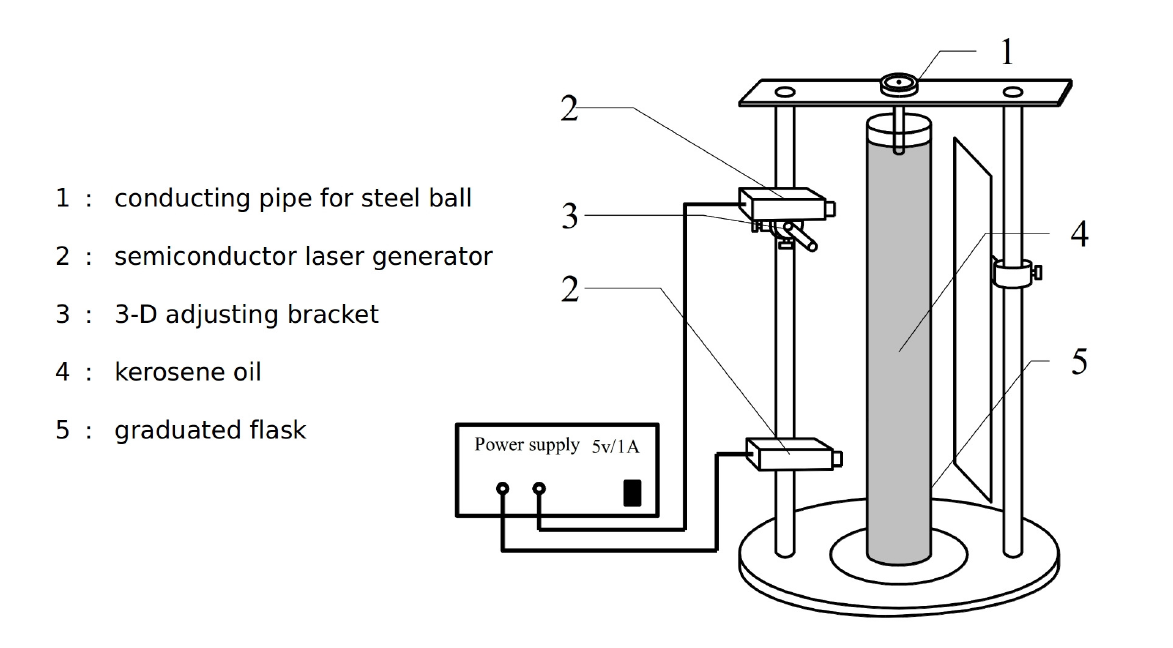
\includegraphics[width=0.5\textwidth]{Apparatus.png}
\caption{Stokes' Viscosity Measurement Apparatus$^{[1]}$}\label{Fig.apparatus}
\end{figure}

\begin{table}[htbp]
\begin{center}
\begin{tabular}{ccc}
\toprule
Device & Quantity Measured & Type-B Uncertainty \\
\midrule
Steel Ruler& Distance between Two Beams & 0.05\,cm\\
Stopwatch& Time Interval the Ball Travels through Beams &0.01\,s\\
Micrometer& Diameter of Metal Ball &  0.005\,mm\\
Calliper& Inner Diameter of Graduated Cylinder & 0.02\,mm\\
Densimeter& Density of Caster Oil &  0.0005\,g/cm$^{3} $\\
Electronic Scale& Mass of Metal Ball &  0.001\,g\\
Thermometer& Ambient Temperature &  0.2\,$^\circ$C\\

\bottomrule
\end{tabular}
\end{center}
\caption{Information of Measurement Devices}\label{Tab.apparatus}
\end{table}



		\section{Measurements Procedure}\label{proc}
\begin{enumerate}

\item Adjustments of the Stokes' viscosity measurement device.

The knobs beneath the base is adjusted so that the plumb aims at the center of the base. The two lasers is turned on and the beams is adjusted until the laser beams are blocked by the string. Then the plumb is removed, and the flask with caster oil is placed at the center of the base. A metal ball is put into the pipe and then whether the ball can block the laser beam when falling downwards in the flask is checked. If it can block the laser beam successfully, the adjustment work is done.
 
\item Measurement of the velocity $v$.

The steel ruler is used to measure the positions of the two beams $x_A$and$x_B$, each for three times. The distance between them is found as $x = x_A - x_B$.
Then, the time spent covering the distance $t$ is found by stopwatch and this step is repeated for six times.
 
\item Measurement of the other quantities.

After measuring the velocity, other quantities are measured using the corresponding devices listed in Table.\ref{Tab.apparatus}.

\item Calculation of $\eta$.

Calculate $\eta$ from Eq.\eqref{Eq.eta} with the data obtained.

\end{enumerate}



		\section{Results}

	\subsection{Distance}
The measured data and the average calculated are presented in Table \ref{Tab.distance}. The distance $x$ is then found to be
\[x = \overline{x_A} - \overline{x_B} = (1.205 \pm 0.007) \times 10^{-1}\,m \]
\begin{table}[htbp]
\centering
\begin{tabular}{cccc}
\toprule
$x_A [\text{cm}] \pm 5\times 10^{-2} [\text{cm}]$  & $x_B [\text{cm}] \pm 5\times 10^{-2} [\text{cm}]$ \\
\hline
21.70 & 9.65 \\
21.70 & 9.65 \\
21.70 & 9.65 \\
\hline
$\overline{x_A}\,$  21.70 & $\overline{x_B}\,$  9.65 \\
\bottomrule
\end{tabular}
\caption{Distance Measurement}\label{Tab.distance}
\end{table}




	\subsection{Time}
The time measured $t$ is shown in Table \ref{Tab.time}. The average time is then found as
\[\overline{t} = \frac{1}{6} \sum \limits_{i=1}^{6} t_i = 4.56 \pm 0.03 \,\text{s}.\]
\begin{table}[htbp]
\centering
\begin{tabular}{cc}
\toprule
time & $t [\text{s}] \pm 0.01 [\text{s}]$\\
\midrule
$t_1$ & 4.58\\
$t_2$ & 4.54\\
$t_3$ & 4.55\\
$t_4$ & 4.60\\
$t_5$ & 4.52\\
$t_6$ & 4.58\\
\bottomrule
\end{tabular}
\caption{Time Measurement}\label{Tab.time}
\end{table}

	\subsection{Diameter of the Ball}
The measured diameter of the ball $d$ is presented in Table \ref{Tab.diameterball}. The average diameter of the balls is then calculated as
\[\overline{d} = \frac{1}{10} \sum \limits_{i=1}^{10} d_i = (1.998 \pm 0.005) \times 10^{-3} \,\text{m}.\]
\begin{table}[htbp]
\centering
\begin{tabular}{cc}
\toprule
diameter & $d [\text{mm}] \pm 0.005 [\text{mm}]$\\
\midrule
$d_1$ & $2.000$\\
$d_2$ & $1.995$\\
$d_3$ & $1.995$\\
$d_4$ & $2.000$\\
$d_5$ & $2.000$\\
$d_6$ & $2.000$\\
$d_7$ & $1.995$\\
$d_8$ & $2.000$\\
$d_9$ & $1.995$\\
$d_{10}$ & $2.000$\\
\bottomrule
\end{tabular}
\caption{Measured Diameters of the Balls}\label{Tab.diameterball}
\end{table}



	\subsection{Inner Diameter of the Flask}
The measurement results of inner diameter $D$ of the flask is showed in Table \ref{Tab.diameterflask}. Then the average of the measured inner diameter of the flask is calculated as
\[\overline{D} = \frac{1}{6} \sum \limits_{i=1}^{6} D_i = (6.161 \pm 0.002)\times 10^{-2}\,\text{m}.\]

\begin{table}[htbp]
\centering
\begin{tabular}{cc}
\toprule
diameter & $D [\text{mm}] \pm 0.02 [\text{mm}]$\\
\midrule
$D_1$ & 61.58\\
$D_2$ & 61.68\\
$D_3$ & 61.54\\
$D_4$ & 61.64\\
$D_5$ & 61.62\\
$D_6$ & 61.60\\
\bottomrule
\end{tabular}
\caption{Measured Inner Diameters of the Flask\label{Tab.diameterflask}}
\end{table}


	\subsection{Other Physical Quantities}
The measurement results of the density of the castor oil, the mass of 40 metal balls, the temperature in the lab and gravitational acceleration in the lab are presented in Table \ref{Tab.data}. The mass of a single ball is then
$$m = m_{40}/40 = (3.285 \pm 0.002) \times 10^{-5}\,\text{kg}$$
\begin{table}[!h]
\centering
\begin{tabular}{ll}
\toprule
Physical Quantities & Values\\
\midrule
Density of the castor oil $\rho_1$ & $0.9550 \pm 0.0005 \,[ \text{g/cm}^3]$\\
Mass of 40 metal balls $m_{40}$& $1.314 \pm 0.001 \,[\text{g}]$\\
Temperature in the lab $T$ &$27.8\pm 0.1 \,[^\circ \text{C}]$\\
Acceleration due to gravity in the lab $g$ & $9.81 \,[\text{m/s}^2]$\\
\bottomrule
\end{tabular}
\caption{Values of Other Physical Quantities}\label{Tab.data}
\end{table}

	\subsection{Viscosity Coefficient}
According to Eq.\eqref{Eq.eta}, the viscosity coefficient of the castor oil can be calculated as
\begin{align*}
\eta &= \frac{(mg-\frac{4}{3}\pi (\frac{d}{2})^3\rho_1g)t}{6\pi x \frac{d}{2}(1+2.4\frac{d}{D})}=\frac{(mg-\frac{1}{6}\pi d^3\rho_1g)t}{3\pi xd(1+2.4\frac{d}{D})}\\
&=\frac{\left[3.285\times10^{-5}\times9.81-\frac{1}{6}\pi (1.998\times10^{-3})^3\times0.9550\times10^{3}\times9.81)\right]\times4.56}{3\pi\times 1.205 \times 10^{-1} \times 1.998 \times 10^{-3} \times (1+2.4\times\frac{1.998\times10^{-3}}{6.161\times10^{-2}})}\\
&= (0.528 \pm 0.003) \, \text{kg}\cdot\text{m}^{-1}\text{s}^{-1},
\end{align*}
with relative uncertainty 0.69\,\%.



		\section{Discussion}
The viscosity coefficient we obtained is
$$\eta = 0.528 \pm 0.003 \, \text{kg}\cdot\text{m}^{-1}\text{s}^{-1} $$
with relative uncertainty 0.69\,\%.

The theoretical viscosity coefficient of castor oil at 28.0 $^\circ$C is 0.49 $\text{kg}\cdot\text{m}^{-1}\text{s}^{-1},^{[2]}$ therefore the relative error of the result is
$$\frac{0.528-0.49}{0.49}\times100\%= 7.76\,\%.$$
The value we measured conforms to the real value to an acceptably degree. Still, Some possible causes for the errors are listed in the following.

\begin{enumerate}
\item The length of the cylinder flask is finite and further corrections to Eq.\eqref{Eq.eta} need considering. This in principle will lead to systematic error.
\item When measure the velocity, it is assumed that the ball has reached constant velocity. However, it needs to be checked whether that is the case$^{[3]}$.
\item The delay due to human's reaction time causes error to time measurement.
\item The metal ball may be deformed by the micrometer during the measurement and causes error.

\end{enumerate}

Some tips for improvement includes:
\begin{enumerate}
\item The adjustment of the apparatus really takes times and effort. It would be better if the cylinder flask is fixed on the device in the proper position.
\item Photoelectric sensor may function better when measuring the time.
\item Further correction due to the finite length can be introduced. According to [4], the factor$\frac{1}{1+1.6\frac{d}{H}}$ can be introduced, where H is the height of the flask.
\end{enumerate}

		\section{Conclusion}
In this lab, the viscosity coefficient of castor oil is measured using Stokes' method. The obtained result is of relatively high accuracy, with relative error of 7.76\,\%	. Some factors that give rise to error may be avoided or reduced in the future improvement.
		
		
		
		\section{Reference}
\noindent [1] Qin Tian, et al. editor.``VP141 Exercise 2: Measurement of Fluid Viscosity''. UM-SJTU Joint Institute. \\
\noindent [2] https://wenku.baidu.com/view/09d23bb1fd0a79563c1e7219.html.\\
\noindent [3] Lin Yuechuan. ``Lab2 guide''. VP141, UM-SJTU Joint Institute. \\
\noindent [4] WANG Ning,LI Xiaoliang,GAO Jingxia, et al. Research on the Deviations of Measurement of Liquid Viscocity Coefficient by Falling-Ball Method[J]. Experiment Science And Technology, 2017, 15(1): 128-130.

\newpage

\appendix

		\section{Measurement Uncertainty Analysis}

	\subsection{Uncertainty of Distance Measurements}
The type-B uncertainty  $\Delta_{x_A,B}= \Delta_{x_B,B} = 0.05 \text{cm} =5 \times 10^{-4} \,\text{m}$. Since the standard deviation
\[s_{\overline{x_A}} =\sqrt{\frac{1}{n-1}\sum \limits_{i=1}^{n}(x_A_,_i-\overline{x_A})^2} = 0\, \text{m}\]
and
\[s_{\overline{x_B}} =\sqrt{\frac{1}{n-1}\sum \limits_{i=1}^{n}(x_B_,_i-\overline{x_B})^2} = 0 \,\text{m}\]
then the type-A uncertainties are found to be
\[\Delta_{x_A,A} = 0\,\text{m},\]
\[\Delta_{x_B,A} = 0\,\text{m}.\]
Thus, the uncertainties of $x_A$ and $x_B$ are
\[u_{x_A} = \sqrt{\Delta_{x_A,A}^2+\Delta_{x_A,B}^2} = \sqrt{(0)^2+(5\times10^{-4})^2} = 5 \times 10^{-4} \,\text{m}.\]
\[u_{x_B} = \sqrt{\Delta_{x_B,A}^2+\Delta_{x_B,B}^2} = \sqrt{(0)^2+(5\times10^{-4})^2} = 5 \times 10^{-4} \,\text{m}.\]
Since the distance \[ s=\overline{x_A}-\overline{x_B},\]
the uncertainty of the distance is calculated according to uncertainty propagation formula
\[u_s = \sqrt{(\frac{\partial s}{\partial x_A})^{2} u_{x_A}^{2}+(\frac{\partial s}{\partial x_B})^{2}  u_{x_B}^{2}} = \sqrt{(1)^2\times(0.0005)^2+(1)^2\times(0.0005)^2} = 7.071 \times 10^{-4} \,\text{m}.\]

	\subsection{Uncertainty of Time Measurements}
The type-B uncertainty $\Delta_{t,B} = 0.01 \text{s}$. The standard deviation is calculated as
$$s_{\overline{t}} =\sqrt{\frac{1}{6-1}\sum \limits_{i=1}^{6}(t_i-\overline{t})^2} = 0.0299 \,\text{s}.$$
With $t_{0.95} = 2.57$ for $n$ = 6, the type-A uncertainty is  
$$\Delta_{t,A} = \frac{2.57}{\sqrt{6}}\times0.0299 = 0.0314 \,\text{s}.$$
The total uncertainty is then
$$u_t = \sqrt{\Delta_{t,A}^2+\Delta_{t,B}^2} = \sqrt{(0.0314)^2+(0.01)^2} = 0.0330 \,\text{s}.$$

	\subsection{Uncertainty of Ball Diameter Measurements}
The type-B uncertainty $\Delta_{d,B} = 0.005\,\text{mm} = 5\times10^{-6}\,\text{m}$. The standard deviation,
$$s_{\overline{d}} =\sqrt{\frac{1}{10-1}\sum \limits_{i=1}^{10}(d_i-\overline{d})^2} = 2.582\times 10^{-3}\,\text{mm}.$$
With $t_{0.95} = 2.26$ for $n$ = 10, the type-A uncertainty is 
$$\Delta_{d,A} = \frac{2.26}{\sqrt{10}}\times2.582\times10^{-3} = 1.845\times10^{-3} \text{mm} = 1.845\times10^{-6} \,\text{m}.$$
The total uncertainty is then
$$u_d = \sqrt{\Delta_{d,A}^2+\Delta_{d,B}^2} = \sqrt{(1.845\times10^{-6})^2+(5\times10^{-6})^2} = 5.330\times10^{-6}\,\text{m}.$$

	\subsection{Uncertainty of Flask Inner Diameter Measurements}
The type-B uncertainty $\Delta_{D,B} = 2\times10^{-5} \,\text{m}$. The standard deviation is calculated as
$$s_{\overline{D}} =\sqrt{\frac{1}{6-1}\sum \limits_{i=1}^{6}(D_i-\overline{D})^2} = 1.18\times 10^{-5}\,\text{m}.$$
With $t_{0.95} = 2.57$ for $n$ = 6, the type-A uncertainty is
$$\Delta_{D,A} = \frac{2.57}{\sqrt{6}}\times1.18\times10^{-5} = 1.23\times10^{-5} \,\text{m}.$$
The total uncertainty is then
$$u_D = \sqrt{\Delta_{D,A}^2+\Delta_{D,B}^2} = \sqrt{(1.23\times10^{-5})^2+(2\times10^{-5})^2} =   2.35\times10^{-5} \,\text{m}.$$

	\subsection{Uncertainty of Other Physical Quantity Measurements}
\begin{enumerate}
\item The measurement of the density of the caster oil is a single measurement with type--$B$ uncertainty of 0.0005 g/cm$^3$. Therefore, its uncertainty is $u_{\rho_1} = 0.0005 \text{g/cm}^3.$
\item The measurement of the mass of 40 metal balls is a single measurement with type--$B$ uncertainty of 10$^{-6}$ kg. Therefore, its uncertainty is $u_{m_{40}} = 10^{-6} \text{kg}$, and the uncertainty of the mass of a single metal ball is $u_m = u_{m_{40}}/40 = 2.5\times10^{-8}$kg.
\item The temperature in the lab is a single measurement with type--$B$ uncertainty of 0.1 $^{\circ}$C. Therefore, its uncertainty is 0.1 $^{\circ}$C.
\item The gravitational acceleration in the lab is a given constant, 9.81 \text{m/$s^2$}, regardless of its uncertainty.
\end{enumerate}

	\subsection{Uncertainty of the Viscosity Coefficient}
Apply uncertainty propagation formula to Eq.\eqref{Eq.eta}, the uncertainty of the viscosity coefficient is
$$ u_\eta=\sqrt{(\frac{\partial \eta}{\partial x})^2(u_x)^2 + (\frac{\partial \eta}{\partial t})^2(u_t)^2 + (\frac{\partial \eta}{\partial d})^2(u_d)^2 + (\frac{\partial \eta}{\partial D})^2(u_D)^2 + (\frac{\partial \eta}{\partial \rho_1})^2(u_{\rho_1})^2 + (\frac{\partial \eta}{\partial m})^2(u_m)^2}.$$
The partial derivatives are calculated below.
\begin{align*}
\frac{\partial \eta}{\partial x} &= -\frac{g}{18}(\frac{6m}{\pi d}-\rho_1 d^2)\frac{t}{x^2}\frac{D}{D+2.4d} = -5.23\, kg  m^{-2} s^{-1}\\
\frac{\partial \eta}{\partial t} &= \frac{g}{18}(\frac{6m}{\pi d}-\rho_1 d^2)\frac{1}{x}\frac{D}{D+2.4d} = 1.04\times10^{-1}\, kg  m^{-1} s^{-2}\\
\frac{\partial \eta}{\partial d} &= -\frac{gD}{18}(\frac{6m}{\pi}\frac{D+4.8d}{d^2(D+2.4d)^2}-\rho_1\frac{2Dd+2.4d^2}{(D+2.4d)^2})\frac{t}{x} = -4.02 \times 10^{2} \, kg m^{-2} s^{-1}\\
\frac{\partial \eta}{\partial D} &= \frac{g}{18}(\frac{6m}{\pi d}-\rho_1 d^2)\frac{t}{x} \frac{2.4d}{(D+2.4d)^2} = 1.20\times 10^{-3}\, kg  m^{-2} s^{-1}\\
\frac{\partial \eta}{\partial \rho_1} &= -\frac{g}{18}\frac{td^2}{x} \frac{D}{D+2.4d} = -9.83\times 10^{-5}\, m^2 s^{-1}\\
\frac{\partial \eta}{\partial m} &= \frac{g}{18}(\frac{6}{\pi d})\frac{t}{x} \frac{D}{D+2.4d} = 2.033\times 10^4\, m^{-1}s^{-1}\\
\end{align*}

Combining the above formulae, the uncertainty of the viscosity coefficient is then found to be
$$u_{\eta} = 3.64\times10^{-3} \,\text{kg}\cdot\text{m}^{-1}\text{s}^{-1},$$
and the relative uncertainty 
$$u_{r\eta} = \frac{u_\eta}{\eta}\times 100\% = \frac{3.64\times 10^{-3}}{0.528} \times 100 \% = 0.69 \%.$$

		\section{Data Sheet}
See the last two pages.

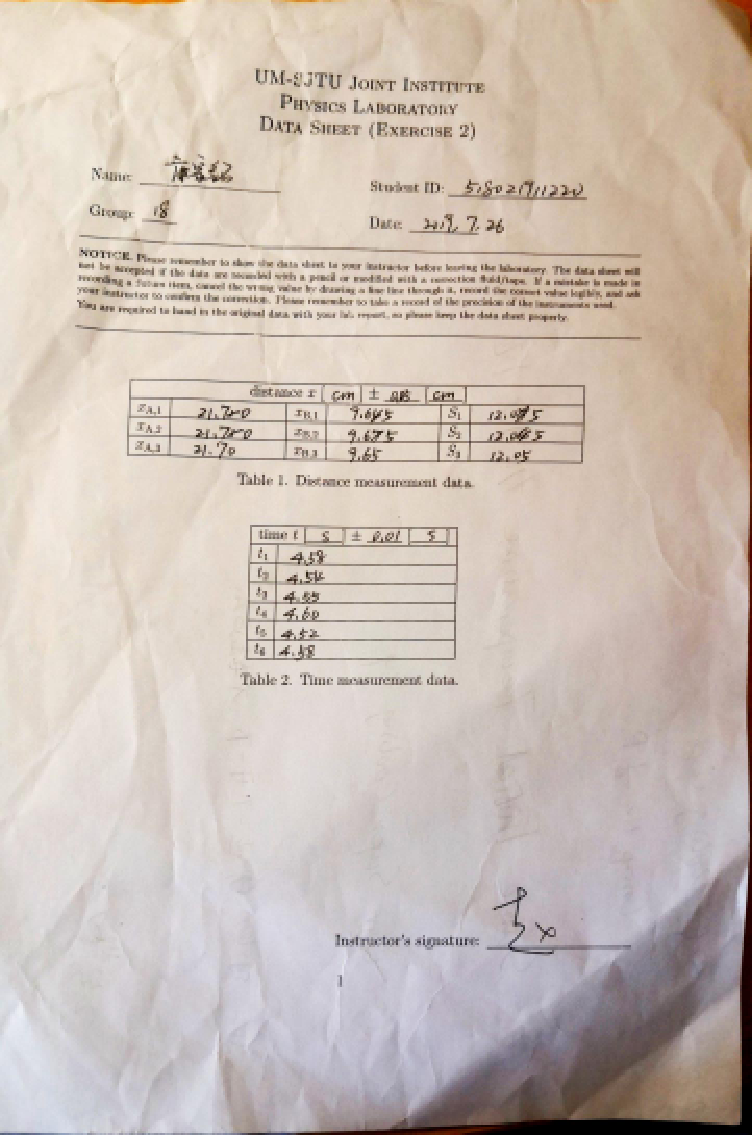
\includepdf[pages=-]{lab2datasheet.pdf}


\end{document}